\section{Solución propuesta}

La telerobótica es el área de la robótica que se ocupa del control de robots a distancia mediante enlaces de comunicación, en general inalámbricos (Wi-Fi, Bluetooth, radiofrecuencia dedicada, etc.). La idea es que un operador humano maneje un dispositivo mecánico situado en un lugar diferente, a veces peligroso o de difícil acceso. Para ello se usan interfaces de control que capturan los movimientos del operador y los replican sobre el robot.

La base de este proyecto es sensar los movimientos de una mano humana y replicarlos, de forma inalámbrica, en una mano impresa en 3D. Los movimientos que se replican son:

\begin{itemize}
    \item Apertura y cierre de cada uno de los cinco dedos, de forma individual.
    \item Rotación de la muñeca (pronosupinación).
    \item Desplazamiento vertical de la mano (flexión y extensión de la muñeca).
\end{itemize}

El sistema se divide en dos nodos, cada uno basado en un microcontrolador ESP32 (placa NodeMCU-32S):

\begin{itemize}
    \item \textbf{Transmisor (guante):} un potenciómetro por dedo, accionado por el movimiento del dedo, y una unidad de medición inercial MPU6050 sobre el dorso de la mano para medir la orientación de la muñeca.
    \item \textbf{Receptor (mano robótica):} cinco servomotores SG90 para los dedos y dos servomotores MG946R para la muñeca.
\end{itemize}

Ambos nodos se comunican mediante ESP-NOW, un protocolo de Espressif que permite enviar paquetes cortos directamente entre placas ESP32 identificadas por su dirección MAC, sin necesidad de un router ni de una red Wi-Fi \cite{espnow_idf}.

Para los dedos se utilizan servos SG90: en este proyecto no se contempla que la mano ejerza fuerza sobre objetos, por lo que alcanza con servos de bajo torque y dimensiones reducidas, que entran dentro de la palma. Para la rotación y el desplazamiento vertical de la muñeca se utilizan servos MG946R, de mayor torque, ya que deben mover el peso de toda la mano. El receptor debe alimentarse con una fuente capaz de entregar la potencia que requieren el microcontrolador y los siete servos (ver sección~\ref{sec:alimentacion}).

\begin{figure}[H]
 \centering
  \subfigure[ESP32]{
    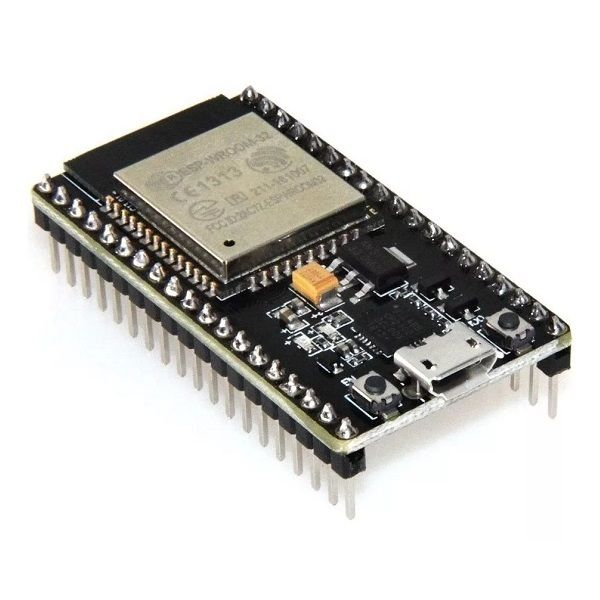
\includegraphics[width=0.2\textwidth]{ESP32.jpeg}}
  \subfigure[SG90]{
    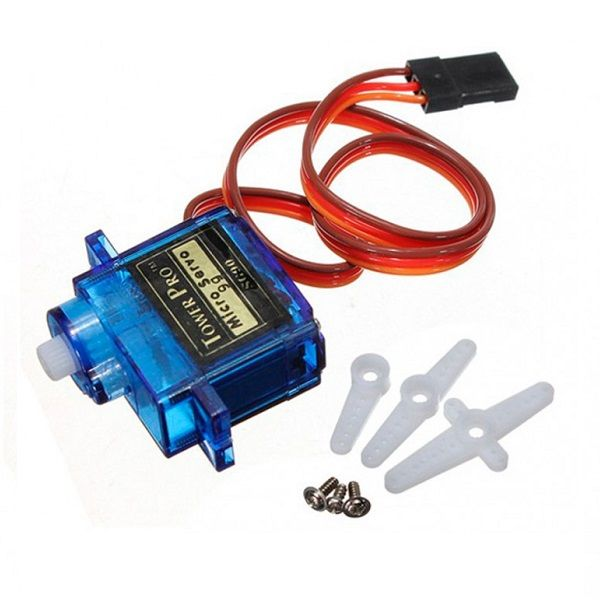
\includegraphics[width=0.2\textwidth]{SG90.jpeg}}
  \subfigure[MG946R]{
    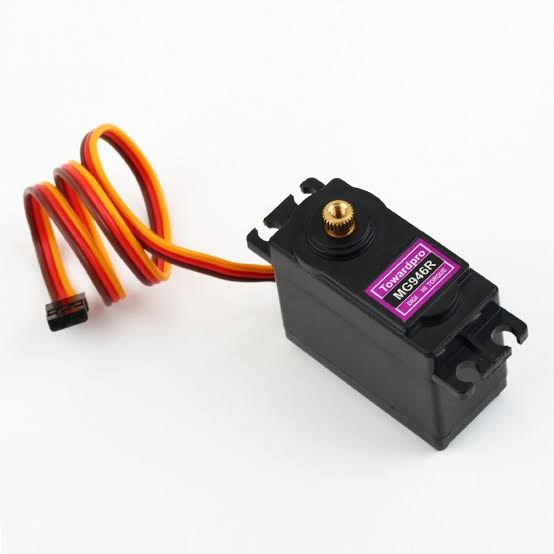
\includegraphics[width=0.2\textwidth]{MG946R.jpg}}
 \caption{Componentes principales del receptor.}
 \label{f:Receptor}
\end{figure}

En el transmisor, el movimiento de cada dedo hace girar un potenciómetro, cuya tensión lee el conversor analógico-digital (ADC) del ESP32. Además, el MPU6050 (acelerómetro y giróscopo de tres ejes) permite estimar la inclinación y la rotación de la mano. El sensor debe montarse paralelo al dorso de la mano y bien orientado, ya que un mal posicionamiento introduce un error en la medición; el firmware prevé constantes de ajuste (\textit{trim}) para compensar pequeñas desalineaciones (sección~\ref{sec:mapeo_munieca}).

\begin{figure}[H]
 \centering
  \subfigure[Potenciómetro]{
    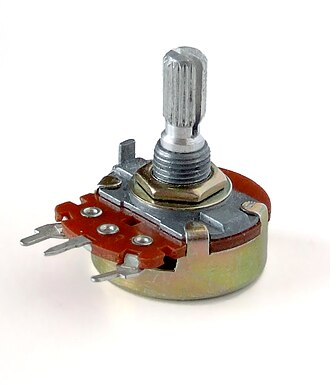
\includegraphics[width=0.2\textwidth]{Potenciometro.jpg}}
  \subfigure[MPU6050]{
    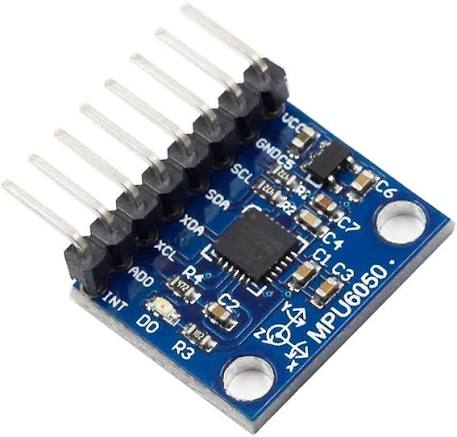
\includegraphics[width=0.2\textwidth]{MPU6050.jpg}}
 \caption{Sensores del transmisor.}
 \label{f:Transmisor}
\end{figure}
